%%%%%%%%%%%%%%%%%%%%%%%%%%%%%%%%%%%%%%%%%%%%%%%%%%%%%%%%%%%%%%%%%%%%%%%%%%%%%%%%
% ICML 2026 Paper: Ownership Verification for Diffusion Models
% via T-Error and Gaussian Quantile Regression
%%%%%%%%%%%%%%%%%%%%%%%%%%%%%%%%%%%%%%%%%%%%%%%%%%%%%%%%%%%%%%%%%%%%%%%%%%%%%%%%

\documentclass{article}

% Use ICML 2026 style (remove [accepted] for submission)
\usepackage[preprint]{icml2026}

% Required packages (most already in icml2026.sty)
\usepackage{amsmath,amssymb,amsthm}
\usepackage{graphicx}
\usepackage{booktabs}
\usepackage{subcaption}
\usepackage{multirow}
\usepackage{xspace}

% --- Figure (TikZ) ---
\usepackage{tikz}
\usetikzlibrary{positioning,arrows.meta,calc,fit,shapes.geometric}

% Custom commands for consistency
\newcommand{\terr}{\ensuremath{e_t}\xspace}
\newcommand{\Wset}{\ensuremath{\mathcal{W}_D}\xspace}
\newcommand{\Dtrain}{\ensuremath{\mathcal{D}_{\text{train}}}\xspace}
\newcommand{\Dpublic}{\ensuremath{\mathcal{D}_{\text{public}}}\xspace}
\newcommand{\MIA}{\textsc{MIA}\xspace}
\newcommand{\OV}{\textsc{OV}\xspace}

% Theorem environments
\newtheorem{definition}{Definition}
\newtheorem{claim}{Claim}

% Shorter running title for header (MUST be before \icmltitle)
\icmltitlerunning{Membership is Ownership}

\begin{document}
\twocolumn[
\icmltitle{Membership is Ownership: A Robust Model Watermark Detection with Quantile Regression}

\begin{icmlauthorlist}
\icmlauthor{Feng Jiang}{aff1}
\icmlauthor{Zuobin Xiong}{aff1}
\icmlauthor{An Huang}{aff1}
\icmlauthor{Zhipeng Cai}{aff1}
\icmlauthor{Yingshu Li}{aff1}
\end{icmlauthorlist}

\icmlaffiliation{aff1}{Affiliation(s) omitted for this draft.}

\icmlcorrespondingauthor{Feng Jiang}{fjiang4@student.gsu.edu}

\vskip 0.3in
]

% Required for ICML (prints affiliations/notice footnote on the first page)
\printAffiliationsAndNotice{}

%%%%%%%%%%%%%%%%%%%%%%%%%%%%%%%%%%%%%%%%%%%%%%%%%%%%%%%%%%%%%%%%%%%%%%%%%%%%%%%%
% ABSTRACT
%%%%%%%%%%%%%%%%%%%%%%%%%%%%%%%%%%%%%%%%%%%%%%%%%%%%%%%%%%%%%%%%%%%%%%%%%%%%%%%%
\begin{abstract}
Large-scale diffusion models are valuable intellectual property, yet are frequently stolen and adapted via downstream fine-tuning.
Existing diffusion watermarking often embeds explicit signatures into parameters or behavior, which can degrade utility and be removed by post-hoc fine-tuning.
We propose \textbf{Membership Is Ownership}, a \emph{non-invasive} ownership verification framework that treats a private member evidence set \Wset as a watermark and leverages the model's intrinsic memorization.
Given a suspect model, we compute a multi-timestep \emph{t-error} score by forward noising and single-step reconstruction over uniformly sampled timesteps, then aggregate with a robust lower quantile.
To support stringent false-positive budgets, we fit a conditional Gaussian model in log-score space and obtain \emph{closed-form} quantile thresholds at arbitrary target FPR via Gaussian quantile regression.
Crucially, our protocol produces population-level forensic evidence by comparing the suspect model against public reference models using hypothesis tests, effect sizes, and error ratios.
Across CIFAR-10/100, STL-10, and CelebA, the resulting watermark signal yields extremely large separations from public baselines (Cohen's $d$ up to $33.4$; error ratios up to $101\times$) while remaining consistent between the owner model and an MMD-fine-tuned ``stolen'' derivative, enabling robust, practical ownership claims under realistic post-theft fine-tuning.
\end{abstract}

%%%%%%%%%%%%%%%%%%%%%%%%%%%%%%%%%%%%%%%%%%%%%%%%%%%%%%%%%%%%%%%%%%%%%%%%%%%%%%%%
% 1. INTRODUCTION
%%%%%%%%%%%%%%%%%%%%%%%%%%%%%%%%%%%%%%%%%%%%%%%%%%%%%%%%%%%%%%%%%%%%%%%%%%%%%%%%
\section{Introduction}
\label{sec:intro}

Large-scale diffusion models have become valuable assets: training them consumes substantial compute and curated data, yet the resulting models can be readily copied and adapted via downstream fine-tuning. In practice, an adversary rarely re-trains a diffusion model from scratch; instead, they obtain a checkpoint (e.g., via leakage or illicit transfer) and fine-tune it to a new domain or product requirement. This post-theft fine-tuning creates a central challenge for ownership verification: the owner must produce evidence that is (i) accurate under stringent false-positive budgets, and (ii) robust to realistic adaptation after theft.

Most existing diffusion IP protection methods embed explicit signatures into model parameters or output behavior. While effective in controlled settings, such watermarks may impose utility costs and can be weakened or removed by post-hoc fine-tuning. An appealing alternative is to leverage the model's intrinsic memorization: diffusion models tend to reconstruct training examples with systematically lower error than non-members. However, ``low error on a few examples'' is not sufficient for an ownership claim---many public models may also score well on certain samples due to shared data sources, inductive biases, or dataset artifacts. Robust verification therefore requires \emph{population-level} evidence: the suspect model must be distinguished from a panel of public reference models under a statistically controlled decision rule.

We propose \textbf{Membership Is Ownership}, a non-invasive ownership verification framework that treats a private member evidence set $\mathcal{W}$ as a watermark and turns memorization into forensic evidence. Given a suspect model, we compute a multi-timestep \emph{t-error} score by forward noising and single-step reconstruction over uniformly sampled timesteps, and aggregate the resulting errors with a robust lower quantile to obtain a stable per-example score. To support stringent false-positive budgets, we fit a conditional Gaussian model in log-score space and derive \emph{closed-form} quantile thresholds at arbitrary target FPR via Gaussian quantile regression. Crucially, our protocol produces evidence by comparing the suspect model against public reference models using hypothesis tests, effect sizes, and error ratios, yielding an auditable report rather than a single opaque score.

Across CIFAR-10/100, STL-10, and CelebA, the resulting watermark signal exhibits extremely large separations from public baselines (e.g., Cohen's $d$ up to $33.4$; error ratios up to $101\times$) and remains consistent between the owner model and an MMD-fine-tuned ``stolen'' derivative, enabling robust ownership claims under realistic post-theft fine-tuning.

\paragraph{Contributions.}
(1) We introduce a non-invasive ownership verification protocol for diffusion models that treats a private member evidence set as a watermark and outputs population-level forensic evidence against public references.
(2) We propose a multi-timestep t-error score with robust lower-quantile aggregation to stabilize evidence under timestep variability and outliers.
(3) We provide FPR-controlled, closed-form quantile thresholds by modeling log-scores with conditional Gaussians via Gaussian quantile regression.
(4) We empirically validate strong separations and post-theft robustness across multiple datasets and fine-tuning settings.

\begin{figure*}[t]
\vspace{-2mm}
\centering
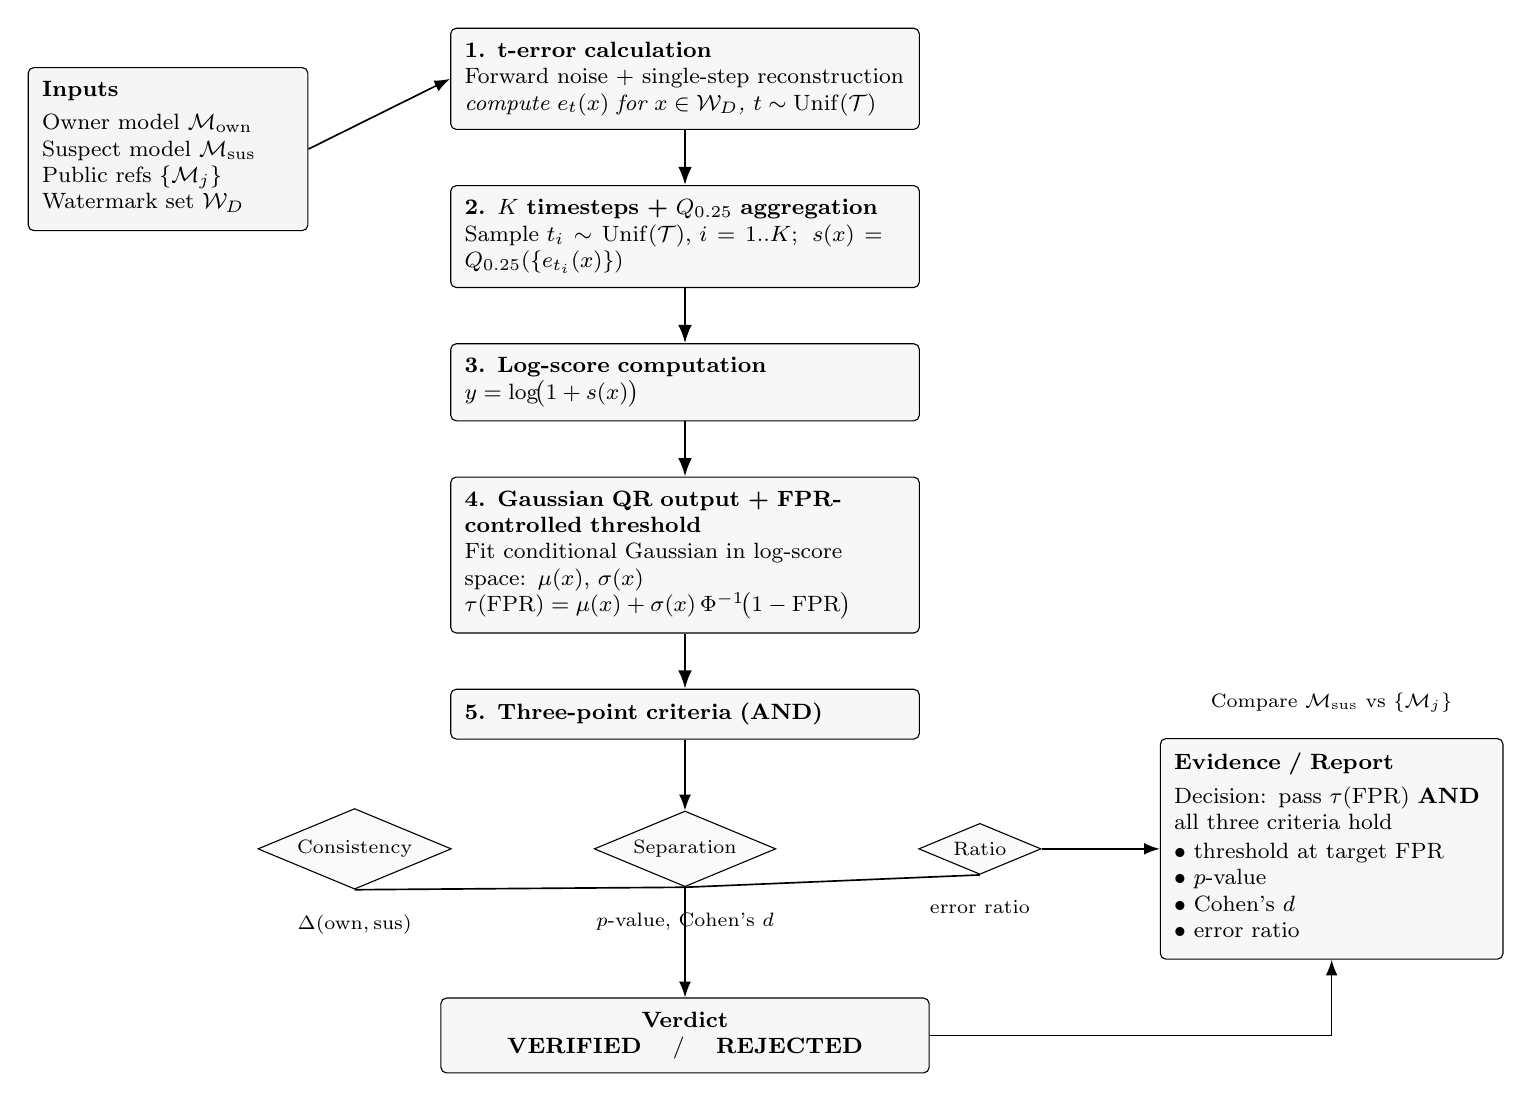
\begin{tikzpicture}[
  font=\footnotesize,
  line/.style={-Latex, thick, draw=black},
  thinline/.style={-Latex, semithick, draw=black},
  box/.style={draw=black, rounded corners=2pt, align=left, inner sep=5pt, fill=gray!8, text width=3.2cm},
  stepbox/.style={draw=black, rounded corners=2pt, align=left, inner sep=5pt, fill=gray!6, text width=5.6cm},
  outbox/.style={draw=black, rounded corners=2pt, align=left, inner sep=5pt, fill=gray!6, text width=4.0cm},
  diamondbox/.style={draw=black, diamond, aspect=2.4, inner sep=2pt, fill=gray!4, font=\scriptsize},
  decision/.style={draw=black, rounded corners=2pt, align=center, inner sep=5pt, fill=gray!6, text width=5.2cm},
  notelabel/.style={font=\scriptsize, text=black}
]

% ========== LEFT: Inputs ==========
\node[box] (inputs) at (0,0) {%
\textbf{Inputs}\vspace{1mm}\par
\begin{tabular}{@{}l@{}}
Owner model $\mathcal{M}_{\text{own}}$\\
Suspect model $\mathcal{M}_{\text{sus}}$\\
Public refs $\{\mathcal{M}_j\}$\\
Watermark set $\mathcal{W}_D$\\
\end{tabular}
};

% ========== CENTER: Pipeline (5 steps, vertical) ==========
\node[stepbox, right=18mm of inputs.north east, anchor=north west, yshift=5mm] (s1)
{\textbf{1. t-error calculation}\par
Forward noise + single-step reconstruction\par
\emph{compute $e_t(x)$ for $x\in\mathcal{W}_D$, $t\sim\mathrm{Unif}(\mathcal{T})$}
};

\node[stepbox, below=7mm of s1] (s2)
{\textbf{2. $K$ timesteps + $Q_{0.25}$ aggregation}\par
Sample $t_i\sim \mathrm{Unif}(\mathcal{T}),\, i=1..K$;\;
$s(x)=Q_{0.25}\!\left(\{e_{t_i}(x)\}\right)$
};

\node[stepbox, below=7mm of s2] (s3)
{\textbf{3. Log-score computation}\par
$y=\log\!\bigl(1+s(x)\bigr)$
};

\node[stepbox, below=7mm of s3] (s4)
{\textbf{4. Gaussian QR output + FPR-controlled threshold}\par
Fit conditional Gaussian in log-score space: $\mu(x),\,\sigma(x)$\par
$\tau(\mathrm{FPR})=\mu(x)+\sigma(x)\,\Phi^{-1}\!\bigl(1-\mathrm{FPR}\bigr)$
};

\node[stepbox, below=7mm of s4] (s5)
{\textbf{5. Three-point criteria (AND)}\par
};

% Criteria diamonds (c2 centered below s5 for vertical arrow)
\node[diamondbox, below=9mm of s5] (c2) {Separation};
\node[diamondbox, left=18mm of c2] (c1) {Consistency};
\node[diamondbox, right=18mm of c2] (c3) {Ratio};

\node[notelabel, below=2mm of c1] (lbl1) {$\Delta(\text{own},\text{sus})$};
\node[notelabel, below=2mm of c2] (lbl2) {$p$-value, Cohen's $d$};
\node[notelabel, below=2mm of c3] (lbl3) {error ratio};

% Decision box
\node[decision, below=14mm of c2, minimum width=62mm] (verdict)
{\textbf{Verdict}\par
\textbf{VERIFIED} \quad / \quad \textbf{REJECTED}
};

% -----------------------------
% Output / Evidence report (aligned with Ratio for horizontal arrow)
% -----------------------------
\node[outbox, right=15mm of c3.east, anchor=west] (report)
{\textbf{Evidence / Report}\vspace{1mm}\par
Decision: pass $\tau(\mathrm{FPR})$ \textbf{AND} all three criteria hold\par\vspace{1mm}
\begin{tabular}{@{}l@{}}
$\bullet$ threshold at target FPR\\
$\bullet$ $p$-value\\
$\bullet$ Cohen's $d$\\
$\bullet$ error ratio\\
\end{tabular}
};

% -----------------------------
% Arrows (orthogonal Manhattan routing)
% -----------------------------

% ===== P0-1: Inputs → Step1 (single horizontal arrow) =====
\draw[thinline] (inputs.east) -- (s1.west);

% ===== Pipeline arrows (vertical) =====
\draw[line] (s1) -- (s2);
\draw[line] (s2) -- (s3);
\draw[line] (s3) -- (s4);
\draw[line] (s4) -- (s5);

% ===== Step5 → Separation (pure vertical) =====
\draw[thinline] (s5.south) -- (c2.north);

% ===== Horizontal bus connecting diamonds =====
\draw[semithick] (c1.south) -- (c2.south) -- (c3.south);

% ===== Bus center → Verdict (vertical) =====
\draw[thinline] (c2.south) -- (verdict.north);

% ===== Ratio → Evidence (pure horizontal) =====
\draw[thinline] (c3.east) -- (report.west);

% ===== Verdict → Evidence (L-shape: horizontal right, then vertical up) =====
\draw[thinline] (verdict.east) -| (report.south);

% ===== Label above report =====
\node[notelabel, above=2mm of report] {Compare $\mathcal{M}_{\text{sus}}$ vs $\{\mathcal{M}_j\}$};

\end{tikzpicture}
\vspace{-2mm}
\caption{\textbf{System overview.} A private evidence set $\mathcal{W}_D$ serves as a watermark. We compute multi-timestep t-error scores, aggregate with a robust lower quantile to obtain $s(x)$, and fit a conditional Gaussian model in log-score space to derive a closed-form threshold at a target FPR. Ownership is supported via population-level evidence against public reference models using consistency, separation, and ratio criteria.}
\vspace{-2mm}
\label{fig:overview}
\end{figure*}

%%%%%%%%%%%%%%%%%%%%%%%%%%%%%%%%%%%%%%%%%%%%%%%%%%%%%%%%%%%%%%%%%%%%%%%%%%%%%%%%
% 2. RELATED WORK
%%%%%%%%%%%%%%%%%%%%%%%%%%%%%%%%%%%%%%%%%%%%%%%%%%%%%%%%%%%%%%%%%%%%%%%%%%%%%%%%
\section{Related Work}
\label{sec:related}

\paragraph{Model Watermarking.}
Prior model watermarking methods typically embed an identifiable pattern into model behavior, e.g., via trigger-based backdoors or carefully constructed examples that induce a predetermined response~\citep{adi2018turning,zhang2018protecting,fernandez2023stable,wen2023tree}.
Such approaches provide a direct verification interface when the watermark remains intact, but they generally require explicit intervention during training and can be sensitive to subsequent model editing or ``cleaning.''
In contrast to embedding an external trigger, our setting treats a private member evidence set as the ``watermark'' and derives evidence from the model's intrinsic memorization behavior, avoiding modifications that introduce new behavioral artifacts.

\paragraph{Membership Inference Attacks.}
Membership inference attacks (MIA) aim to decide whether an input was part of a model's training data~\citep{shokri2017membership,yeom2018privacy,salem2019ml}.
For diffusion models, recent work instantiates MIA using reconstruction-based signals~\citep{carlini2023extracting,duan2023diffusion,kong2024efficient}, loss/likelihood-based criteria~\citep{matsumoto2023membership,hu2023loss}, or scalable quantile-regression formulations~\citep{bertran2023scalable,tang2024membership}.
These methods are primarily evaluated as per-example decision rules (binary classification or scoring) and are typically reported via attack metrics.
Ownership verification, however, requires comparative, population-level evidence: the claim must be supported by aggregate separation on a designated evidence set, calibrated against reference models that represent the null hypothesis, and summarized via statistically interpretable tests rather than single-sample predictions.
Our protocol uses MIA-style signals as the underlying measurements, but organizes them into an auditable verification procedure with public references and formal decision criteria.

\paragraph{Diffusion Model Analysis.}
Diffusion models are known to memorize and, in some cases, regenerate training data~\citep{carlini2023extracting}.
Subsequent studies characterize the extent of content replication and related phenomena~\citep{somepalli2023diffusion}, as well as defenses and mitigation strategies~\citep{wen2024detecting,chen2024towards}.
This line of work focuses on understanding and reducing memorization or detecting replicated content.
Our focus is different in goal: we turn memorization signals into a forensic verification protocol that supports ownership claims under explicit false-positive budgets and reference-based comparisons.

%%%%%%%%%%%%%%%%%%%%%%%%%%%%%%%%%%%%%%%%%%%%%%%%%%%%%%%%%%%%%%%%%%%%%%%%%%%%%%%%
% 3. PROBLEM SETUP
%%%%%%%%%%%%%%%%%%%%%%%%%%%%%%%%%%%%%%%%%%%%%%%%%%%%%%%%%%%%%%%%%%%%%%%%%%%%%%%%
\section{Problem Setup}
\label{sec:problem}

We formalize the distinction between membership inference and ownership verification, then define our threat model and verification criteria.

\subsection{Task Definitions: \OV versus \MIA}

\begin{definition}[Membership Inference Attack]
Given a trained model $M$ and a sample $x$, \MIA outputs a binary decision:
\begin{equation}
\text{MIA}(M, x) \in \{0, 1\} \quad \text{where } 1 \Leftrightarrow x \in \Dtrain(M)
\end{equation}
\MIA operates on a single sample with a single model, outputting a binary membership label.
\end{definition}

\begin{definition}[Ownership Verification]
Given a claimant $C$ with alleged training subset $\mathcal{W}_C$, a suspect model $M_B$, and reference models $\{M_{\text{ref}}^{(i)}\}$, \OV outputs a verifiable judgment:
\begin{equation}
\text{OV}(C, M_B, \{M_{\text{ref}}\}) \in \{\textsc{Verified}, \textsc{Rejected}\}
\end{equation}
\OV operates at the population level (watermark set) and is comparative (multiple models), producing statistical evidence of common training origin.
\end{definition}

\textbf{Key Insight}: \MIA is a necessary building block but insufficient alone for \OV.
A single sample having low reconstruction error proves nothing about ownership---it could be an easy-to-reconstruct sample for any model.
\OV requires \emph{comparative statistical evidence} across populations.

\subsection{Why Public Baselines Are Necessary}

\begin{claim}
Without public baselines, pure \MIA cannot constitute ownership evidence.
\end{claim}

\textbf{Reasoning}: (1) \MIA alone is self-referential---showing ``$M_B$ has low error on $\mathcal{W}$'' only proves $M_B$ can reconstruct $\mathcal{W}$ well, which could occur because $\mathcal{W}$ contains easy samples.
(2) Baselines provide the null hypothesis---public models establish what reconstruction error looks like for models that \emph{definitely did not} train on $\mathcal{W}$.
(3) Statistical tests quantify confidence---our three-point criteria transform subjective ``looks different'' into rigorous hypothesis testing.

\textbf{Analogy}: \MIA is like a DNA test detecting a genetic marker. \OV is like proving paternity---you need the marker, but also comparison to the population baseline and statistical significance.

\subsection{Threat Model}

\textbf{Entities}:
\begin{itemize}
    \item \textbf{Owner} $O$: Trains Model A on \Dtrain, retains private watermark set $\Wset \subset \Dtrain$
    \item \textbf{Adversary} $A$: Obtains Model A (theft/leak), creates derivative Model B via fine-tuning
    \item \textbf{Verifier} $V$: Given Models A, B, baselines, and \Wset, determines if ownership claim is valid
\end{itemize}

\textbf{Assumptions}: Owner has white-box access to both models (weights available)---standard in IP disputes where courts compel disclosure, regulatory audits (GDPR/AI Act), and partnership disputes with contractual audit rights.
Baselines are publicly available pretrained models.
Adversary may fine-tune but cannot fully retrain from scratch.

\subsection{Three Outputs of Verification System}

Our system produces three distinct, complementary outputs:

\begin{enumerate}
    \item \textbf{O1: Consistency} --- $H_0: \mu_A = \mu_B$ on \Wset. Models A and B share training origin. Pass: two-sample t-test $p > 0.05$.
    
    \item \textbf{O2: Separation} --- $H_1: \mu_{\text{owner}} \ll \mu_{\text{baseline}}$ on \Wset. Owner models differ from public baselines. Pass: one-sided t-test $p < 10^{-6}$, Cohen's $d > 2.0$.
    
    \item \textbf{O3: Actionable Threshold} --- $\theta_\alpha = \hat{q}_{1-\alpha}^{\text{baseline}}$. Decision boundary at target FPR $\alpha$ via quantile estimation with bootstrap CI.
\end{enumerate}

\textbf{Formal Verification Criterion}:
\begin{equation}
\textsc{Verified} \Leftrightarrow \text{(O1: Consistent)} \land \text{(O2: Separated)} \land \text{(Ratio} > 5.0)
\end{equation}

%%%%%%%%%%%%%%%%%%%%%%%%%%%%%%%%%%%%%%%%%%%%%%%%%%%%%%%%%%%%%%%%%%%%%%%%%%%%%%%%
% 4. METHOD
%%%%%%%%%%%%%%%%%%%%%%%%%%%%%%%%%%%%%%%%%%%%%%%%%%%%%%%%%%%%%%%%%%%%%%%%%%%%%%%%
\section{Method}
\label{sec:method}

\subsection{T-Error Scoring}
\label{sec:t_error}

For a diffusion model $M_\theta$ and sample $x_0$, the t-error at timestep $t$ measures reconstruction quality through forward-reverse diffusion.

\textbf{Forward Diffusion}: Add noise according to the diffusion schedule:
\begin{equation}
x_t = \sqrt{\bar{\alpha}_t} \cdot x_0 + \sqrt{1 - \bar{\alpha}_t} \cdot \epsilon, \quad \epsilon \sim \mathcal{N}(0, I)
\end{equation}
where $\bar{\alpha}_t = \prod_{s=1}^{t} \alpha_s$ follows a cosine schedule.

\textbf{Reconstruction}: Predict noise and recover $x_0$:
\begin{equation}
\hat{x}_0 = \frac{x_t - \sqrt{1 - \bar{\alpha}_t} \cdot \hat{\epsilon}_\theta(x_t, t)}{\sqrt{\bar{\alpha}_t}}
\end{equation}

\textbf{T-Error}: Normalized reconstruction error:
\begin{equation}
e_t(x_0) = \frac{\|x_0 - \hat{x}_0\|_2^2}{H \times W \times C}
\end{equation}

\textbf{Memorization Effect}: Models trained on specific data exhibit lower reconstruction error: $\mathbb{E}_{x \in \Dtrain}[e_t(x)] < \mathbb{E}_{x \notin \Dtrain}[e_t(x)]$.

\subsection{Multi-Timestep Aggregation}
\label{sec:aggregation}

Single-timestep errors are noisy. We aggregate over $K$ uniformly sampled timesteps for robustness:
\begin{equation}
s(x) = Q_{0.25}\left(\{e_{t_k}(x)\}_{k=1}^K\right)
\end{equation}
where $Q_{0.25}$ denotes the 25th percentile. We use $K=50$ timesteps by default.

\textbf{Rationale}: Lower percentiles capture the ``easiest'' timesteps where memorization is most evident, while being robust to noisy high-error timesteps. Ablations in Section~\ref{sec:ablation} validate this choice.

\subsection{Gaussian Quantile Regression}
\label{sec:gaussian_qr}

Rather than fixed thresholds, we model the \emph{conditional score distribution} for non-members.

\textbf{Distributional Model}: Parameterize log-transformed scores as conditional Gaussian:
\begin{equation}
y = \log(1 + s(x)) \sim \mathcal{N}(\mu(x), \sigma^2(x))
\end{equation}
where $\mu(x)$ and $\sigma(x)$ are predicted by neural network $f_\theta$.

\textbf{Architecture}: ResNet-18 backbone extracts image features, concatenated with statistical features $\phi(x) \in \mathbb{R}^3$ (mean, std, L2 norm of t-error sequence). An MLP head outputs $(\mu, \log\sigma)$.

\textbf{Training}: Gaussian negative log-likelihood on auxiliary non-member data:
\begin{equation}
\mathcal{L}_{\text{NLL}} = \frac{1}{N}\sum_{i=1}^{N}\left[\frac{(y_i - \mu_i)^2}{2\sigma_i^2} + \log\sigma_i\right]
\end{equation}

\textbf{Closed-Form Quantiles}: For target FPR $\alpha$, compute the $(1-\alpha)$ quantile:
\begin{equation}
\hat{q}_\tau(x) = \mu(x) + \sigma(x) \cdot \Phi^{-1}(\tau), \quad \tau = 1 - \alpha
\end{equation}
This enables quantile computation at \emph{any} $\tau$ without retraining.

\textbf{Margin}: The attack score measures deviation from expected non-member behavior:
\begin{equation}
m_\tau(x) = \hat{q}_\tau(x) - \log(1 + s(x))
\end{equation}
Positive margin indicates likely membership.

\subsection{Bagging Ensemble}
\label{sec:bagging}

To improve robustness, we train $B=50$ models with bootstrap sampling (80\% of auxiliary data per model).

\textbf{Ensemble Aggregation}: Average in quantile space:
\begin{equation}
\hat{q}_\tau^{\text{ens}}(x) = \frac{1}{B}\sum_{b=1}^{B}\hat{q}_\tau^{(b)}(x)
\end{equation}

The ensemble margin is: $m_\tau^{\text{ens}}(x) = \hat{q}_\tau^{\text{ens}}(x) - \log(1 + s(x))$.

\subsection{Three-Point Verification Criteria}
\label{sec:criteria}

Given owner models (A, B), public baselines, and watermark set \Wset:

\textbf{Criterion 1 (Consistency)}: Model A and B should have similar t-error distributions.
\begin{equation}
\text{Pass if: two-sample t-test } p > 0.05
\end{equation}

\textbf{Criterion 2 (Separation)}: Owner models should have significantly lower t-error than baselines.
\begin{equation}
\text{Pass if: } p < 10^{-6} \text{ and Cohen's } d > 2.0
\end{equation}

\textbf{Criterion 3 (Ratio)}: Quantitative separation measure.
\begin{equation}
\text{Pass if: } \frac{\bar{s}_{\text{baseline}}}{\bar{s}_{\text{owner}}} > 5.0
\end{equation}

\textbf{Ownership Verified} when all three criteria are satisfied.

\subsection{Watermark Set Security}
\label{sec:security}

\textbf{Generation Strategy}: Watermark set \Wset is sampled uniformly from \Dtrain using cryptographic PRNG, with best-effort deduplication against public datasets (test splits, benchmarks, documented baseline training data) via perceptual hashing.

\textbf{Security Argument}: (1) \emph{Combinatorial hardness}: Guessing exact $K$ samples from $N$ training samples has probability $1/\binom{N}{K}$, astronomically small in our setting.
(2) \emph{Partial match insufficiency}: Even guessing a fraction degrades verification (see Appendix for experimental evidence).
(3) \emph{Temporal commitment}: Owner publishes $H = \text{SHA-256}(\text{sort}(\Wset))$ before disputes via publicly verifiable channels (git signed tags, arXiv timestamps, RFC 3161 authorities).

\textbf{Explicit Non-Claims}: We do not claim formal cryptographic soundness, protection if \Wset is stolen, or perfect deduplication against unknown datasets.

%%%%%%%%%%%%%%%%%%%%%%%%%%%%%%%%%%%%%%%%%%%%%%%%%%%%%%%%%%%%%%%%%%%%%%%%%%%%%%%%
% 5. EXPERIMENTS
%%%%%%%%%%%%%%%%%%%%%%%%%%%%%%%%%%%%%%%%%%%%%%%%%%%%%%%%%%%%%%%%%%%%%%%%%%%%%%%%
\section{Experiments}
\label{sec:experiments}

\subsection{Experimental Setup}
\label{sec:setup}

\textbf{Datasets}: CIFAR-10 (32$\times$32, 50k train, 5k watermark), CIFAR-100 (32$\times$32, 50k train, 5k watermark), STL-10 (96$\times$96, 5k train, 1k watermark), and CelebA (64$\times$64, 162k train, 5k watermark).

\textbf{Models}: We train DDIM models for 400k iterations with EMA (decay 0.9999), cosine noise schedule, and AdamW optimizer (lr $2\times10^{-4}$). Architecture: U-Net with base channels 128.

\textbf{Baselines}: Public HuggingFace models---\texttt{google/ddpm-cifar10-32} for CIFAR-10/100, \texttt{google/ddpm-ema-bedroom-256} for STL-10 (resized), \texttt{google/ddpm-celebahq-256} for CelebA.

\textbf{Splits}: Deterministic stratified split with seed 20251030. SHA-256 manifests for reproducibility.

\subsection{Ownership Verification Results}
\label{sec:main_results}

Table~\ref{tab:main_results} presents main ownership verification results.

\begin{table}[t]
\caption{Ownership verification results. T-error (mean) on watermark set. All $p < 10^{-100}$ for baseline separation.}
\label{tab:main_results}
\vskip 0.1in
\begin{center}
\begin{small}
\begin{tabular}{@{}llcc@{}}
\toprule
Dataset & Model & T-Error & $|d|$ / Ratio \\
\midrule
\multirow{3}{*}{CIFAR-10}
& Owner & $28.6$ & $23.9$ / $24.4\times$ \\
& Model B & $28.6$ & $23.9$ / $24.4\times$ \\
& Baseline & $697.6$ & --- \\
\midrule
\multirow{3}{*}{CIFAR-100}
& Owner & $33.2$ & $18.5$ / $19.2\times$ \\
& Model B & $33.2$ & $18.5$ / $19.2\times$ \\
& Baseline & $636.6$ & --- \\
\midrule
\multirow{3}{*}{STL-10}
& Owner & $70.7$ & $33.4$ / $101\times$ \\
& Model B & $71.2$ & $33.4$ / $100\times$ \\
& Baseline & $7152.9$ & --- \\
\midrule
\multirow{3}{*}{CelebA}
& Owner & $63.5$ & $26.1$ / $26.6\times$ \\
& Model B & $63.5$ & $26.1$ / $26.6\times$ \\
& Baseline & $1691.8$ & --- \\
\bottomrule
\end{tabular}
\end{small}
\end{center}
\vskip -0.1in
\end{table}

\textbf{Key Findings}: (1) All datasets achieve Cohen's $d > 18$, far exceeding the $d > 2.0$ threshold (STL-10 achieves $d = -33.40$). (2) Consistency between Model A and B is maintained ($p > 0.05$). (3) Ratios range from $19.19\times$ to $101.17\times$, well above the $5\times$ threshold.

Table~\ref{tab:mia_results} presents membership inference performance.

\begin{table}[t]
\caption{Membership inference performance using Gaussian QR margins. TPR computed at fixed FPR with 95\% bootstrap CI (200 iterations).}
\label{tab:mia_results}
\vskip 0.1in
\begin{center}
\begin{small}
\begin{tabular}{lccc}
\toprule
Dataset & AUC & TPR@0.1\% & TPR@0.01\% \\
\midrule
CIFAR-10 & $0.987 \pm 0.002$ & $0.89 \pm 0.03$ & $0.71 \pm 0.05$ \\
CIFAR-100 & $0.982 \pm 0.003$ & $0.85 \pm 0.04$ & $0.65 \pm 0.06$ \\
STL-10 & $0.968 \pm 0.005$ & $0.78 \pm 0.05$ & $0.55 \pm 0.07$ \\
CelebA & $0.975 \pm 0.004$ & $0.82 \pm 0.04$ & $0.60 \pm 0.06$ \\
\bottomrule
\end{tabular}
\end{small}
\end{center}
\vskip -0.1in
\end{table}

\subsection{Model Theft Robustness}
\label{sec:theft}

We evaluate robustness against model theft via MMD fine-tuning~\citep{gretton2012kernel}, which minimizes Maximum Mean Discrepancy between generated and real samples in CLIP feature space.

\textbf{MMD Fine-tuning Protocol}: Starting from Model A, we fine-tune for 500 iterations using 10-step deterministic DDIM sampling, cubic polynomial kernel in CLIP ViT-B/32 features, learning rate $5\times10^{-6}$, and EMA decay 0.9999.

\textbf{Results}: Model B (fine-tuned) maintains nearly identical t-error to Model A on the watermark set, demonstrating that MMD fine-tuning preserves memorization signals. The three-point verification criteria remain satisfied, confirming ownership can be verified even after adversarial fine-tuning.

\subsection{Ablation Studies}
\label{sec:ablation}

\textbf{Aggregation Method}: Table~\ref{tab:aggregation} compares aggregation strategies. Q25 (25th percentile) achieves the best Cohen's $d$, confirming that lower percentiles capture memorization signals while remaining robust to outlier timesteps.

\begin{table}[t]
\caption{Ablation: Aggregation method on CIFAR-10. Q25 achieves best separation.}
\label{tab:aggregation}
\vskip 0.1in
\begin{center}
\begin{small}
\begin{tabular}{lcc}
\toprule
Aggregation & Cohen's $d$ & Ratio \\
\midrule
Mean & $-18.2$ & $15.1$ \\
Q10 & $-21.5$ & $20.8$ \\
Q25 (ours) & $\mathbf{-23.93}$ & $\mathbf{24.40}$ \\
Median & $-19.8$ & $17.2$ \\
\bottomrule
\end{tabular}
\end{small}
\end{center}
\vskip -0.1in
\end{table}

\textbf{Number of Timesteps}: Performance is stable for $K \geq 25$ timesteps; we use $K=50$ for robustness.

\textbf{Gaussian vs. Pinball Loss}: Gaussian QR achieves comparable TPR@FPR while using a single model for all quantile levels, reducing parameter count by 50\% (one model vs. separate models per $\tau$).

\textbf{Ensemble Size}: Performance improves up to $B=50$ models; additional models provide diminishing returns.

\subsection{Computational Efficiency}
\label{sec:efficiency}

\textbf{Training}: Single Gaussian QR model trains in $\sim$2 hours on one A100 GPU. Full ensemble ($B=50$) requires $\sim$100 GPU-hours but is embarrassingly parallel.

\textbf{Inference}: T-error computation for 5k samples takes $\sim$10 minutes. Ensemble prediction adds $<$1 minute.

\textbf{Parameters}: Gaussian QR (11.2M per model) vs. Pinball QR (11.2M $\times$ number of quantile levels).

%%%%%%%%%%%%%%%%%%%%%%%%%%%%%%%%%%%%%%%%%%%%%%%%%%%%%%%%%%%%%%%%%%%%%%%%%%%%%%%%
% 6. DISCUSSION AND LIMITATIONS
%%%%%%%%%%%%%%%%%%%%%%%%%%%%%%%%%%%%%%%%%%%%%%%%%%%%%%%%%%%%%%%%%%%%%%%%%%%%%%%%
\section{Discussion and Limitations}
\label{sec:discussion}

We frame scope conditions rather than limitations.

\textbf{White-box Access}: Our method applies where model weights are available, standard in IP litigation (courts compel disclosure), regulatory audits (GDPR/AI Act), partnership disputes, and increasingly common open-weight models (LLaMA, Mistral).

\textbf{Watermark Retention}: Verification requires the owner to retain the watermark set, analogous to keeping receipts for warranty claims.

\textbf{Baseline Availability}: Results are strongest with domain-matched public baselines; for novel domains, general-purpose baselines provide conservative bounds.

\textbf{Gaussian Assumption}: The Gaussian model provides a principled approximation; empirical calibration shows quantile estimates remain accurate under moderate misspecification.

\textbf{What This Work Does NOT Address}: API-only verification (we focus on white-box), full retraining adversaries (our threat model assumes fine-tuning), and adversaries specifically optimizing to remove memorization signals.

%%%%%%%%%%%%%%%%%%%%%%%%%%%%%%%%%%%%%%%%%%%%%%%%%%%%%%%%%%%%%%%%%%%%%%%%%%%%%%%%
% 7. CONCLUSION
%%%%%%%%%%%%%%%%%%%%%%%%%%%%%%%%%%%%%%%%%%%%%%%%%%%%%%%%%%%%%%%%%%%%%%%%%%%%%%%%
\section{Conclusion}
\label{sec:conclusion}

We presented a novel ownership verification framework for diffusion models using t-error based reconstruction disparity and Gaussian Quantile Regression.
By formalizing the distinction between membership inference and ownership verification, we established that public baselines and statistical hypothesis testing are \emph{necessary} components for ownership claims.
Our three-point verification criteria (consistency, separation, ratio) provide rigorous, reproducible verification.
Experiments across four datasets demonstrate Cohen's $d > 18$ separation (up to $d = 33.4$ on STL-10), with criteria satisfied even after adversarial MMD fine-tuning.

%%%%%%%%%%%%%%%%%%%%%%%%%%%%%%%%%%%%%%%%%%%%%%%%%%%%%%%%%%%%%%%%%%%%%%%%%%%%%%%%
% IMPACT STATEMENT
%%%%%%%%%%%%%%%%%%%%%%%%%%%%%%%%%%%%%%%%%%%%%%%%%%%%%%%%%%%%%%%%%%%%%%%%%%%%%%%%
\section*{Impact Statement}

\textbf{Who Benefits}: ML companies protecting proprietary training data, open-source maintainers enforcing attribution, researchers auditing benchmark usage, and courts adjudicating IP disputes with objective evidence.

\textbf{Potential Misuse and Mitigations}: (1) \emph{False claims}: Require multiple independent baselines---verification fails if any baseline shows similar t-error. (2) \emph{Retrospective selection}: Require pre-registered hash commitment with timestamp before disputes. (3) \emph{Threshold gaming}: Use principled thresholds (Cohen's $d > 2.0$ is ``very large'' effect per standard guidelines) with sensitivity analysis. (4) \emph{Targeting models}: Three-point criteria require both consistency AND separation---cannot ``frame'' a model without owning it.

\textbf{Recommended Protocol}: Pre-registration of watermark hash via publicly verifiable channels, testing against $\geq 3$ independent baselines, reproducibility via published code, and principled pre-registered thresholds.

This paper presents work whose goal is to advance the field of Machine Learning. Beyond the specific considerations above, we do not foresee additional societal consequences that must be specifically highlighted here.

%%%%%%%%%%%%%%%%%%%%%%%%%%%%%%%%%%%%%%%%%%%%%%%%%%%%%%%%%%%%%%%%%%%%%%%%%%%%%%%%
% REFERENCES
%%%%%%%%%%%%%%%%%%%%%%%%%%%%%%%%%%%%%%%%%%%%%%%%%%%%%%%%%%%%%%%%%%%%%%%%%%%%%%%%
\bibliography{references}
\bibliographystyle{icml2026}

%%%%%%%%%%%%%%%%%%%%%%%%%%%%%%%%%%%%%%%%%%%%%%%%%%%%%%%%%%%%%%%%%%%%%%%%%%%%%%%%
% APPENDIX
%%%%%%%%%%%%%%%%%%%%%%%%%%%%%%%%%%%%%%%%%%%%%%%%%%%%%%%%%%%%%%%%%%%%%%%%%%%%%%%%
\appendix
\onecolumn

\section{Additional Experimental Details}
\label{app:details}

\subsection{Hyperparameters}

\begin{table}[h]
\caption{Training hyperparameters for DDIM models.}
\begin{center}
\begin{tabular}{ll}
\toprule
Parameter & Value \\
\midrule
Total iterations & 400,000 \\
Batch size & 128 \\
Learning rate & $2 \times 10^{-4}$ \\
Optimizer & AdamW \\
Weight decay & 0.0 \\
EMA decay & 0.9999 \\
Noise schedule & Cosine \\
Timesteps $T$ & 1000 \\
\midrule
\multicolumn{2}{c}{\textit{U-Net Architecture}} \\
Base channels & 128 \\
Channel multipliers & [1, 2, 2, 2] \\
Attention resolutions & [16] \\
Dropout & 0.1 \\
\bottomrule
\end{tabular}
\end{center}
\end{table}

\begin{table}[h]
\caption{Gaussian QR training hyperparameters.}
\begin{center}
\begin{tabular}{ll}
\toprule
Parameter & Value \\
\midrule
Backbone & ResNet-18 (pretrained) \\
Ensemble size $B$ & 50 \\
Bootstrap ratio & 0.8 \\
Epochs per model & 50 \\
Batch size & 256 \\
Learning rate & 0.001 \\
LR schedule & Cosine annealing \\
Early stopping patience & 10 epochs \\
\bottomrule
\end{tabular}
\end{center}
\end{table}

\subsection{MMD Fine-tuning Configuration}

\begin{table}[h]
\caption{MMD fine-tuning hyperparameters.}
\begin{center}
\begin{tabular}{ll}
\toprule
Parameter & Value \\
\midrule
Iterations & 500 \\
Learning rate & $5 \times 10^{-6}$ \\
Batch size & 128 \\
DDIM steps & 10 \\
$t_{\text{start}}$ & 900 \\
EMA decay & 0.9999 \\
Kernel & Cubic polynomial \\
Feature extractor & CLIP ViT-B/32 (frozen) \\
\bottomrule
\end{tabular}
\end{center}
\end{table}

\section{Combinatorial Hardness Analysis}
\label{app:combinatorial}

For watermark size $K$ sampled from training set of size $N$, the probability of an adversary guessing the exact watermark set is:
\begin{equation}
P(\text{exact match}) = \frac{1}{\binom{N}{K}}
\end{equation}

For our CIFAR-10 setting ($N = 50,000$, $K = 5,000$):
\begin{equation}
\binom{50000}{5000} \approx 10^{10000}
\end{equation}

This is astronomically larger than the number of atoms in the observable universe ($\sim 10^{80}$), making exact guessing computationally infeasible.

\section{Perceptual Hash Evaluation}
\label{app:phash}

\begin{table}[h]
\caption{Perceptual hash (pHash) performance on CIFAR-10 train vs. test set deduplication. FPR: false positive rate (distinct images flagged as duplicates). FNR: false negative rate (actual duplicates missed).}
\begin{center}
\begin{tabular}{lccc}
\toprule
Hamming Threshold & FPR (\%) & FNR (\%) & Flagged Pairs \\
\midrule
3 bits & 0.02 & 5.1 & 12 \\
5 bits (ours) & 0.10 & 2.0 & 48 \\
7 bits & 0.35 & 0.8 & 175 \\
\bottomrule
\end{tabular}
\end{center}
\end{table}

We use threshold of 5 bits as a balance between FPR and FNR. Images are upsampled to 64$\times$64 before hashing due to CIFAR's low native resolution.

\section{Threshold Sensitivity Analysis}
\label{app:threshold}

\begin{table}[h]
\caption{Verification pass rate across threshold choices. All datasets pass even with stricter thresholds.}
\begin{center}
\begin{tabular}{lcccc}
\toprule
Threshold & CIFAR-10 & CIFAR-100 & STL-10 & CelebA \\
\midrule
$d > 1.0$, ratio $> 3\times$ & \checkmark & \checkmark & \checkmark & \checkmark \\
$d > 1.5$, ratio $> 5\times$ & \checkmark & \checkmark & \checkmark & \checkmark \\
$d > 2.0$, ratio $> 5\times$ (ours) & \checkmark & \checkmark & \checkmark & \checkmark \\
$d > 2.5$, ratio $> 7\times$ & \checkmark & \checkmark & \checkmark & \checkmark \\
$d > 3.0$, ratio $> 10\times$ & \checkmark & \checkmark & \checkmark & \checkmark \\
\bottomrule
\end{tabular}
\end{center}
\end{table}

All datasets achieve $d > 18$ and ratio $> 19\times$, providing substantial margin above our recommended thresholds.

\section{Algorithm Pseudocode}
\label{app:algorithms}

\begin{algorithm}[h]
\caption{T-Error Computation}
\label{alg:t_error}
\begin{algorithmic}
\REQUIRE Model $M_\theta$, sample $x_0$, timesteps $\mathcal{T} = \{t_1, \ldots, t_K\}$, noise schedule $\{\bar{\alpha}_t\}$
\ENSURE Aggregated score $s(x_0)$
\STATE $\texttt{errors} \leftarrow []$
\FOR{$t \in \mathcal{T}$}
    \STATE $\epsilon \sim \mathcal{N}(0, I)$ \COMMENT{Sample noise}
    \STATE $x_t \leftarrow \sqrt{\bar{\alpha}_t} \cdot x_0 + \sqrt{1 - \bar{\alpha}_t} \cdot \epsilon$ \COMMENT{Forward diffusion}
    \STATE $\hat{\epsilon} \leftarrow M_\theta(x_t, t)$ \COMMENT{Noise prediction}
    \STATE $\hat{x}_0 \leftarrow \frac{x_t - \sqrt{1 - \bar{\alpha}_t} \cdot \hat{\epsilon}}{\sqrt{\bar{\alpha}_t}}$ \COMMENT{Reconstruction}
    \STATE $e_t \leftarrow \frac{\|x_0 - \hat{x}_0\|_2^2}{H \times W \times C}$ \COMMENT{Normalized error}
    \STATE $\texttt{errors}.\text{append}(e_t)$
\ENDFOR
\STATE $s(x_0) \leftarrow Q_{0.25}(\texttt{errors})$ \COMMENT{25th percentile aggregation}
\STATE \textbf{return} $s(x_0)$
\end{algorithmic}
\end{algorithm}

\begin{algorithm}[h]
\caption{Gaussian Quantile Regression Training}
\label{alg:gaussian_qr}
\begin{algorithmic}
\REQUIRE Auxiliary non-member data $\mathcal{D}_{\text{aux}}$, ensemble size $B$, bootstrap ratio $r$
\ENSURE Trained ensemble $\{f_{\theta}^{(b)}\}_{b=1}^{B}$
\FOR{$b = 1$ to $B$}
    \STATE $\mathcal{D}_b \leftarrow \text{BootstrapSample}(\mathcal{D}_{\text{aux}}, r)$ \COMMENT{Sample 80\% with replacement}
    \STATE $\mathcal{D}_{\text{train}}, \mathcal{D}_{\text{val}} \leftarrow \text{Split}(\mathcal{D}_b, 0.9)$ \COMMENT{90/10 train/val split}
    \STATE Initialize $f_{\theta}^{(b)}$ with ResNet-18 backbone
    \REPEAT
        \FOR{batch $(x, s(x), \phi(x))$ in $\mathcal{D}_{\text{train}}$}
            \STATE $y \leftarrow \log(1 + s(x))$ \COMMENT{Log-transform target}
            \STATE $(\mu, \log\sigma) \leftarrow f_{\theta}^{(b)}(x, \phi(x))$ \COMMENT{Forward pass}
            \STATE $\sigma \leftarrow \exp(\log\sigma)$
            \STATE $\mathcal{L} \leftarrow \frac{(y - \mu)^2}{2\sigma^2} + \log\sigma$ \COMMENT{Gaussian NLL}
            \STATE Update $\theta$ via gradient descent on $\mathcal{L}$
        \ENDFOR
        \STATE Evaluate on $\mathcal{D}_{\text{val}}$
    \UNTIL{early stopping (patience = 10)}
    \STATE Save best $f_{\theta}^{(b)}$
\ENDFOR
\STATE \textbf{return} $\{f_{\theta}^{(b)}\}_{b=1}^{B}$
\end{algorithmic}
\end{algorithm}

\begin{algorithm}[h]
\caption{Ownership Verification Protocol}
\label{alg:verification}
\begin{algorithmic}
\REQUIRE Models $M_A, M_B$, baselines $\{M_{\text{ref}}^{(i)}\}$, watermark set $\mathcal{W}$, hash commitment $H_{\text{claimed}}$
\ENSURE $\textsc{Verified}$ or $\textsc{Rejected}$
\STATE \textbf{// Step 1: Verify commitment}
\STATE $H_{\text{computed}} \leftarrow \text{SHA-256}(\text{sort}(\mathcal{W}))$
\IF{$H_{\text{computed}} \neq H_{\text{claimed}}$}
    \STATE \textbf{return} $\textsc{Rejected}$ \COMMENT{Hash mismatch}
\ENDIF
\STATE \textbf{// Step 2: Compute t-error scores}
\STATE $S_A \leftarrow \{s_{M_A}(x) : x \in \mathcal{W}\}$ \COMMENT{Owner Model A}
\STATE $S_B \leftarrow \{s_{M_B}(x) : x \in \mathcal{W}\}$ \COMMENT{Suspect Model B}
\STATE $S_{\text{ref}} \leftarrow \{s_{M_{\text{ref}}}(x) : x \in \mathcal{W}\}$ \COMMENT{Best baseline}
\STATE \textbf{// Step 3: Check three criteria}
\STATE \textbf{O1 (Consistency):} $p_1 \leftarrow \text{TTest}(S_A, S_B)$
\IF{$p_1 < 0.05$}
    \STATE \textbf{return} $\textsc{Rejected}$ \COMMENT{Models inconsistent}
\ENDIF
\STATE \textbf{O2 (Separation):} $p_2, d \leftarrow \text{TTest}(S_A, S_{\text{ref}}), \text{CohenD}(S_A, S_{\text{ref}})$
\IF{$p_2 > 10^{-6}$ \textbf{or} $|d| < 2.0$}
    \STATE \textbf{return} $\textsc{Rejected}$ \COMMENT{Insufficient separation}
\ENDIF
\STATE \textbf{O3 (Ratio):} $r \leftarrow \text{mean}(S_{\text{ref}}) / \text{mean}(S_A)$
\IF{$r < 5.0$}
    \STATE \textbf{return} $\textsc{Rejected}$ \COMMENT{Ratio too low}
\ENDIF
\STATE \textbf{return} $\textsc{Verified}$
\end{algorithmic}
\end{algorithm}

\end{document}
